\documentclass[10pt]{article}
\usepackage{amsmath}
\usepackage{graphicx}
\usepackage[vspacewithsolns,
%    coverpage,coverpagesumry=byparts,
    pointsonboth,totalsonright,forpaper]{eqexam}

\title[T2]{Test 2}
\author{D. P. Story}
\subject[C1]{Calculus I}
\date{Spring \the\year}
\keywords{Test~2, Section 001}

\university
{%
      THE UNIVERSITY OF AKRON\\
    Theoretical and Applied Mathematics
}
\email{dpstory@uakron.edu}

\solAtEndFormatting{\eqequesitemsep{3pt}}


\begin{document}

\maketitle

\begin{exam}[Part I.]{Part1}

\begin{instructions}[Part I.]
Solve each of the problems without error. If you make an error,
points will be subtracted from your total score.
\end{instructions}


\begin{problem}[5]
This is an example of a objective question, the student fills in his/her response
in the space below.

\begin{solution}[.5in]
The solution to the question. This solution will not appear when
the option \texttt{nosolutions} is specified. It will appear
immediately after the question with the \texttt{solutionsafter}
option, and appear at the end of the document if a solutions
option is not specified.
\end{solution}
\end{problem}


\begin{problem}[5]
An example of a fill-in question:
It is well known that \fillin{1in}{Newton} and
\fillin{1in}{Leibniz} are jointly credited as the founders of
modern calculus.

\begin{solution}
It is well known that \underbar{Newton} and \underbar{Leibniz} are
jointly credited as the founders of modern calculus.

\medskip\noindent\textbf{Notes.} Here the optional argument for
the \texttt{solution} environment is not specified, this implies
that no room should be left for the student to answer, seems
reasonable since this is a fill-in.
\end{solution}
\end{problem}

\begin{problem*}[3ea]
\textit{True} or \textit{False}.  No justification needed.

% Comment out this next line to see the effect.
\fillinWidth\defaultTFwidth

\begin{parts}

    \item[h] \TF{T} If triangles have $4$ sides, then all monkeys
    are green. Now is the time for all good men to come to the aid
    of their country.

\begin{solution}
    This is the solution, let's hope it's correct, or I would be embarrassed to no end.
    Now is the time for all good men to come to the aid
    of their country.

    \medskip\noindent\textbf{Notes.} This \texttt{\string\item}
    has an optional argument `\texttt{[h]}', so the
    solution will not appear at the end of the document when there
    is no solutions option, but will appear when
    \texttt{solutionsafter} is specified. The
    \texttt{nohiddensolutions} option can override this feature.
\end{solution}

    \item[H] \TF{T} $1+1=3$ iff $\sqrt2$ is a rational number. Now is the time for all good men to come to the aid
    of their country.

\begin{solution}
    \textbf{Notes.} This \texttt{\string\item} has an optional argument `\texttt{[H]}', so
    the solution will not appear at the end of the document when there is no solutions option, nor does
    it appear when \texttt{solutionsafter} is specified. The
    \texttt{noHiddensolutions} option can override this feature.
\end{solution}

    \item[h] \TF{F} $(\forall x)(\exists y)(xy>1)$\hskip1em($x$, $y$~real numbers). Now is the time for all good men to come to the aid
    of their country.

    \item[h] \TF{F} $(\forall x)(\exists y)(\forall z)(z(x+y)>0)$,
        \hskip1em($x$,~$y$, and~$z$ real numbers).

%\end{exam}
%\end{document}




\end{parts}
\end{problem*}



\begin{problem*}[\auto]
Here is an example of a auto calculate problem. It takes the optional
argument `\texttt{[\string\auto]}'. You specify the points associated with each part
using the \texttt{\string\PTs} command.

\begin{parts}

\item \PTs{10} This a hard one!

\begin{solution}[1in]
This is a tough solution.
\end{solution}

\item \PTs{5} This one is ``half'' as hard.

\begin{solution}[1in]
This solution is easy.
\end{solution}

\end{parts}
\end{problem*}

\begin{problem*}[\auto]\sqForms
Select the correct answer for each of the following multiple choice. There is
only one correct answer.
\begin{parts}
    \item\PTs{5} In what year did Columbus sail the ocean blue?
    \begin{answers}{6} % specify 6 columns for a tabular environment
    \Ans0 1490 &\Ans0 1491 &\Ans1 1492 &\Ans0 1493
    \end{answers}
\begin{solution}
Yes, Columbus sailed the ocean blue in 1492.
\end{solution}

    \item\PTs{6} In what year did Columbus sail the ocean blue?
    \begin{answers}{1} % specify a list environment.
    \Ans0 1490
    \Ans0 1491
    \Ans1 1492
    \Ans0 1493
    \end{answers}
\begin{solution}
Yes, Columbus sailed the ocean blue in 1492.
\end{solution}

\end{parts}
\end{problem*}


\begin{problem}[5]
Which of the following best describes Augustin Cauchy?

\sqForms % change this multiple choice to a forms style.

\begin{multicols}{2}

% use two columns

\begin{answers}{1} % an argument of 1 means list style

\Ans0 He developed the Calculus while his University was closed
for the plague.  % Newton
\Ans0 Given credit for first using the functional notation
$f(x)$. % Euler
\Ans0 He created the ``bell-shaped curve'' and first used the
method of least squares.  % Gauss

\Ans1 He first formulated a precise definition of the limit
and continuity of a function.  % Cauchy
\Ans0 Gave a rigorous definition of the definite integral---an
integral that now bears his name.  % Riemann
\Ans0 His notation for the derivative and the integral is used
even to this day. % Leibniz

\end{answers}
\end{multicols}


\begin{solution}
This is a solution to a problem question.
\end{solution}

\end{problem}

\begin{problem}[3]
This is a question.  Work \OnBackOfPage, and be quick about it!

\begin{solution}[1in]
This is the solution, let's hope it's correct, or I would be embarrassed to no end.
\end{solution}
%
% This example illustrates the use of the work area. Place the
% \texttt{workarea} environment just below the \texttt{solution} environment, it's
% parameter must be the same as the one specified by \texttt{solution}. The material
% in the \texttt{workarea} environment will lay on top the vertical space generated above,
% when the \texttt{nosoutions} option is specified; otherwise, it does nothing.
%
\begin{workarea}[.5\linewidth]{1in}
Peter piper picked a peck of pickled peppers, how many pecks of pickled
peppers did Peter Piper pick?
%
\vfill\hfill\setlength{\fboxsep}{6pt}\fbox{Answer: \fillin[b]{1in}{17}}
\end{workarea}
\end{problem}

\begin{problem}[7]
This is a question. Now is the time for all good men to come to
the aid of their country. Peter Piper picked a peck of pickled
peppers. Use the figure below.


\begin{solution}[1in]
This a really good  solution. I hope this solution is correct or I will be
embarrassed to no end. Even if it is wrong, maybe the students will appreciate
my effort. You can see from the figure that the solution is obvious.
(You could also use commands from a figure wrapping package as well.)
\end{solution}
\begin{workarea}[\linewidth]{1in}
\hfill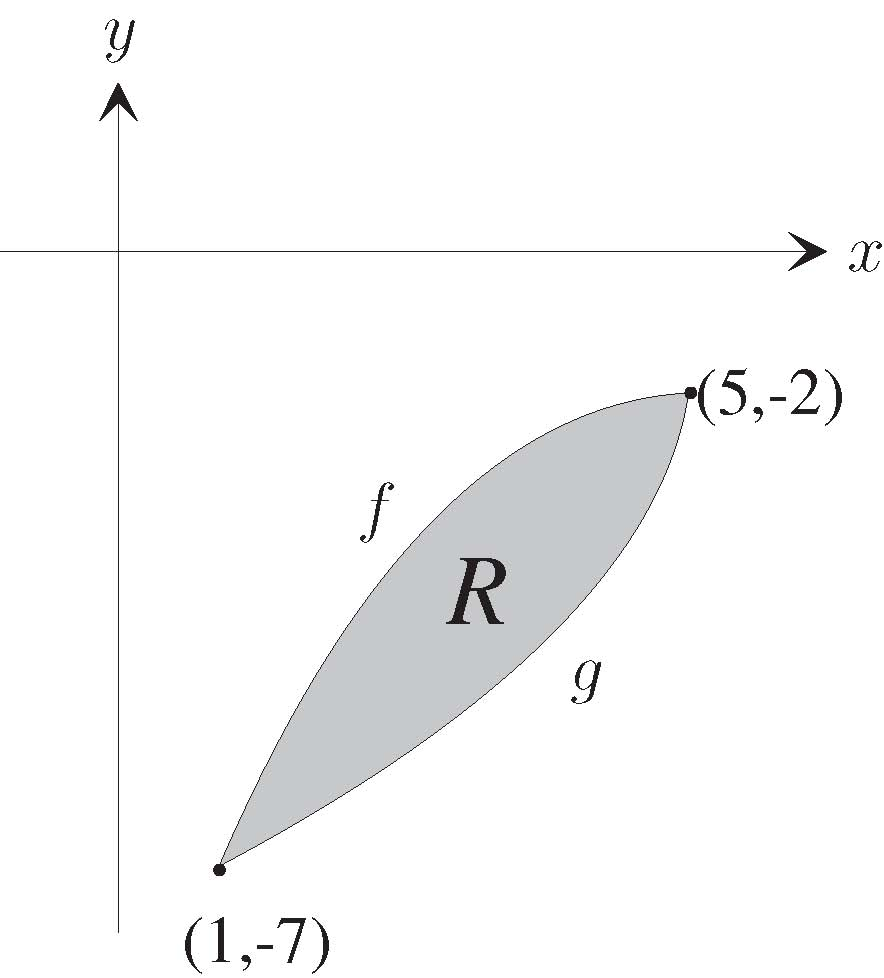
\includegraphics[scale=.2]{fig1}
\end{workarea}
\end{problem}

% The previous solution works well for paper publications, however, when the online
% or email option is taken, a text field is created for the student to type into,
% the graphics and text are superimposed on top this text field, so the student
% types over these elements, not a good solution in this case.
%
% The next example illustrates a work around. It works for both paper and for online
% documents.

\begin{problem}[5]
This is a question worth $5$ points.

\begin{solution}[1.5in]
This a really good  solution. I hope this solution is correct or I will be total
embarrassed to no end. Even if it is wrong, maybe the students will appreciate
my tremendous effort. You can see from the figure that the solution is obvious.
\end{solution}
\end{problem}

% This example illustrates multiple part a question

\begin{problem*}[10ea]
Answer each of the following questions.
\begin{parts}
\item This is a question.
\begin{solution}[1in]
Now is the time for all good men to come to the aid of their country.
Now is the time for all good men to come to the aid of their country.
Now is the time for all good men to come to the aid of their country.
\end{solution}
\item This is a question.
\begin{solution}[1in]
Now is the time for all good men to come to the aid of their country.
Now is the time for all good men to come to the aid of their country.
Now is the time for all good men to come to the aid of their country.
\end{solution}
\end{parts}
\end{problem*}

% This example illustrates multiple part a question using the multicol package

\begin{problem*}[12]
Solve each of the following. Work \OnBackOfPage
\begin{multicols}{2}

\def\solnsp{1in}

\begin{parts}
\item This is a question.  Be sure you don't make any error, I'm watching.

\begin{solution}[\solnsp]
This is the solution.
\end{solution}

\item This is a question.
\begin{solution}[\solnsp]
This is the solution.
\end{solution}

\item This is a question.
\begin{solution}[\solnsp]
This is the solution.
\end{solution}

\item This is a question.
\begin{solution}[\solnsp]
This is the solution.
\end{solution}
\end{parts}
\end{multicols}
\end{problem*}

\end{exam}

\begin{exam}[Part II.]{Part2}

\begin{instructions}[Part II.]
The following is a short review of previously mastered material.
\end{instructions}

\begin{problem}[5]
This is a question.
\begin{solution}[.5in]
This is the solution to answer all questions.
\end{solution}
\end{problem}

\begin{problem}[7]
This is a question.
\begin{solution}[.5in]
This is the solution to answer all questions.
\end{solution}
\end{problem}

\begin{problem}[8]
This is a question.
\begin{solution}[1in]
This is the solution to answer all questions.
\end{solution}
\end{problem}

\begin{problem}[5]
This is a question.
\begin{solution}[1in]
This is the solution to answer all questions.
\end{solution}
\end{problem}

\begin{problem}[10]
This is a question.
\begin{solution}[1in]
This is the solution to answer all questions.
\end{solution}
\end{problem}

\begin{problem}[5]
This is a question.
\begin{solution}[1in]
This is the solution to answer all questions.
\end{solution}
\end{problem}

\begin{problem}[10]
This is a question.
\begin{solution}[1in]
This is the solution to answer all questions.
\end{solution}
\end{problem}
\end{exam}

\end{document}
